\section{РЕЗУЛЬТАТЫ ЖАНРОВОЙ КЛАССИФИКАЦИИ}
\label{sec:genre_classification}


Для проверки значимости выделенных образов было принято решения проверить их на задаче жанровой классификации. 

В качестве исходной выборки был использован репозиторий GZTAG. Набор данных состоит из 1000 звуковых дорожек каждые по 30 секунд. Он содержит 10 жанров, каждый из которых представлен 100 треками. Все треки - это все 220-мегагерцовые Mono 16-битные аудиофайлы в формате .wav.


Для решения задачи классификации была использована библиотека scikit-learn -- бесплатная библиотека для машинного обучения с открытым исходным кодом для языка программирования Python. Все методы классификации использованы с параметрами по умолчанию. 

\subsection{AdaBoost с деревьями принятия решений}

AdaBoost zвляется мета-алгоритмом, в процессе обучения строит композицию из базовых алгоритмов обучения для улучшения их эффективности. AdaBoost является алгоритмом адаптивного бустинга в том смысле, что каждый следующий классификатор строится по объектам, которые плохо классифицируются предыдущими классификаторами.

AdaBoost вызывает слабый классификатор в цикле. После каждого вызова обновляется распределение весов, которые отвечают важности каждого из объектов обучающего множества для классификации. На каждой итерации веса каждого неверно классифицированного объекта возрастают, таким образом новый классификатор <<фокусирует своё внимание>> на этих объектах.

В качестве слабого классификаторы было использованно дерево принятие решений. Максимальное количество слабых классификаторов установлено в количестве 50. В качестве алгоритма обучения использовался алгоритм SAMME.


Как показывает рисунок \ref{fig:results:adaboost} данный классификатор плохо справляется с задачей классификации. Классифицировались фрагменты по 5 секунд с перекрытием в 0,5 секунд. Из жанров лучше всего классифицировались классическая музыка -- 70 \%, металл -- 47 \% и хипхоп -- 49 \%. 

Оценка перекрёстной проверки с десятью разбиениями -- 28 \% cо средней квадратичным отклонением 3,8 \%.  

Для задачи жанровой классификации данный метод с текущими параметрами и с теми выделенными образами для решения задачи жанровой классификации не подходит. 

\begin{figure}[h]
\centering
  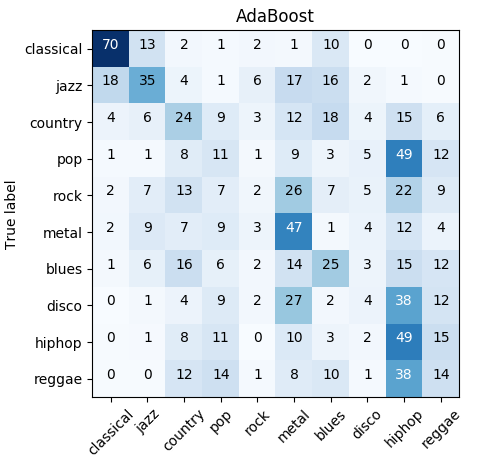
\includegraphics{AdaBoost.png}
  \caption{Матрица ошибок полученная с помощь метода классификации AdaBoost SAMME, где используется <<комитет>>  деревьев принятия решений.}
  \label{fig:results:adaboost}
\end{figure}

\subsection{Дерево принятия решений}

Деревья принятия решений - это непараметрический контролируемый метод обучения, используемый для классификации и регрессии. Цель состоит в том, чтобы создать модель, которая предсказывает значение целевой переменной путем изучения простых правил принятия решений, выведенных из данных.

В качестве алгоритма обучения используется оптимизированная версия CART. В качестве индекса неоднородности используется индекс Джини. Максимальная глубина дерева ограничена до 5 уровней.

Как показывает рисунок \ref{fig:results:DecisionTree} дерево принятия решений смогло выделить все классы, что видно по главной диагонали матрицы ошибок. Лучше всего распознались следующие жанры: классическая музыка -- 61 \%, джаз -- 56 \%, поп -- 50 \% и метал -- 58 \%. Хуже всего: диско -- 29 \%, рок -- 25 \%. 


Оценка перекрёстной проверки с десятью разбиениями -- 42 \% cо средней квадратичным отклонением 4 \%.  

\begin{figure}[h]
\centering
  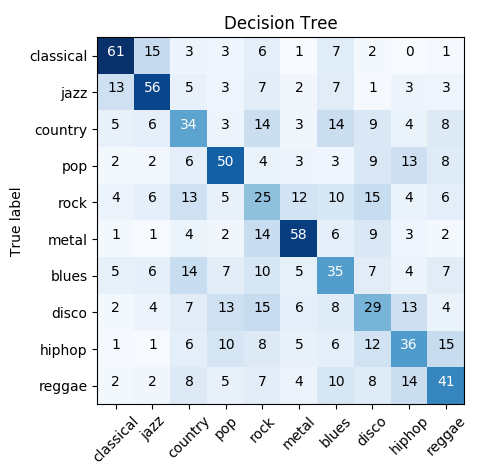
\includegraphics{DecisionTree.png}
  \caption{Матрица ошибок полученная с помощь дерева принятия решения}
  \label{fig:results:DecisionTree}
\end{figure}

При классификации всего трека использовалась интегрированная оценка по всем фрагментам. Класс трека определялся наиболее часто встречаемым предсказанным классом его фрагментов. Это улучшило результаты классификации, как можно видеть на рисунке \ref{fig:results:DecisionTree1}. 

\begin{figure}[h]
\centering
  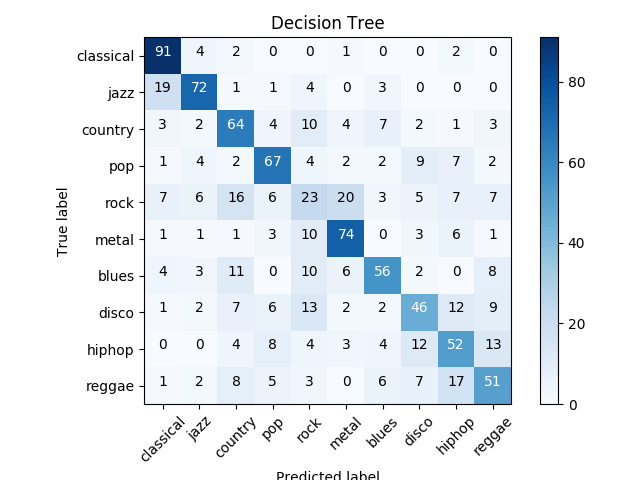
\includegraphics{DecisionTree_new1.png}
  \caption{Матрица ошибок полученная с помощь дерева принятия решения}
  \label{fig:results:DecisionTree1}
\end{figure}


\subsection{Метод опорных векторов}


\begin{figure}[h]
\centering
  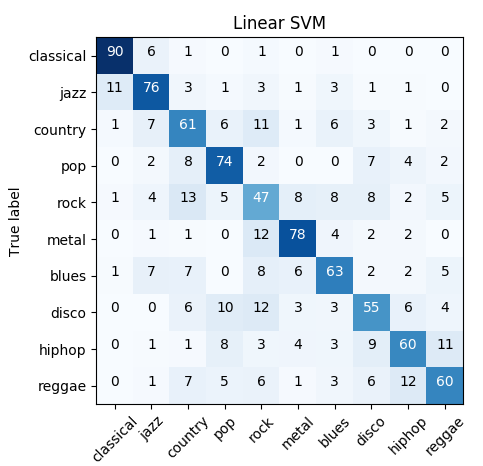
\includegraphics{LinearSVM.png}
  \caption{Матрица ошибок полученная с помощь метода опорных векторов}
  \label{fig:results:LinearSVM}
\end{figure}



\subsection{Наивный баесовский классификатор}

\begin{figure}[h]
\centering
  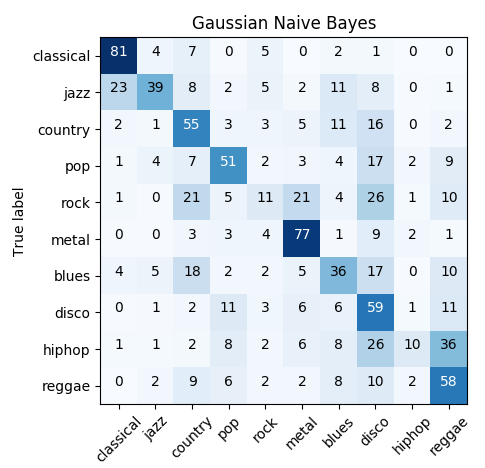
\includegraphics{NaiveBayes.png}
  \caption{Матрица ошибок полученная с помощь наивного баесовского классификатора}
  \label{fig:results:NaiveBayes}
\end{figure}


\subsection{Метод ближайших соседей}

Метод k ближайших соседей -- метрический алгоритм для автоматической классификации объектов. Основным принципом метода ближайших соседей является то, что объект присваивается тому классу, который является наиболее распространённым среди соседей данного элемента.

Соседи берутся исходя из множества объектов, классы которых уже известны, и, исходя из ключевого для данного метода значения k высчитывается, какой класс наиболее многочислен среди них. Каждый объект имеет конечное количество атрибутов (размерностей).

Предполагается, что существует определенный набор объектов с уже имеющейся классификацией.

\begin{figure}[h]
\centering
  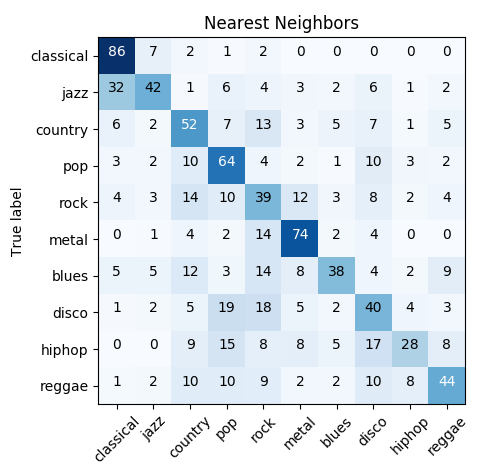
\includegraphics{NearestNeighbors.png}
  \caption{Матрица ошибок полученная с помощь метода k ближайших соседей}
  \label{fig:results:NearestNeighbors}
\end{figure}

\subsection{Нейронная сеть прямого распространения}

\begin{figure}[h]
\centering
  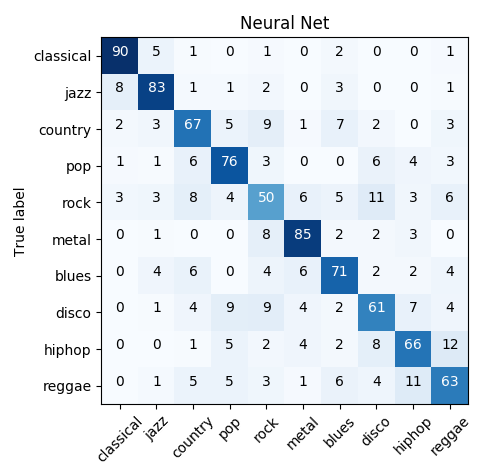
\includegraphics{NeuralNet.png}
  \caption{Матрица ошибок полученная с помощь многослойного перцептрона}
  \label{fig:results:NeuralNet}
\end{figure}


\subsection{Квадратичный дискриминант}


Квадратичный дискриминант - это вариант Байесовского классификатора, который основывается на двух дополнительных допущениях, касающихся вероятностных свойств выборки, а именно - независимость выборки и ее нормальность. Нормальное (гауссово) распределение широко используется по причине вычислительного удобства и адекватности во многих случаях. 

\begin{figure}[h]
\centering
  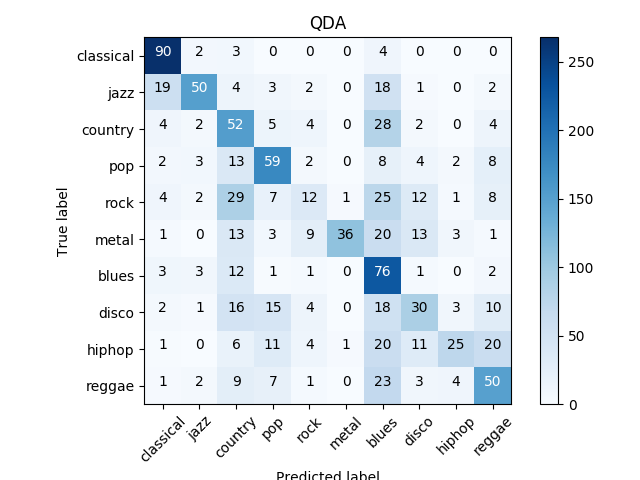
\includegraphics{QDA.png}
  \caption{Матрица ошибок полученная с помощь QDA}
  \label{fig:results:QDA}
\end{figure}


\subsection{Случайный лес}

\begin{figure}[h]
\centering
  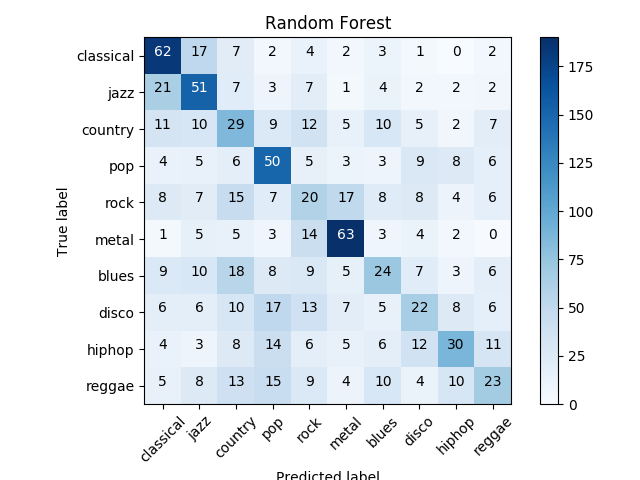
\includegraphics{RandomForest.png}
  \caption{Матрица ошибок полученная с случайного леса}
  \label{fig:results:RandomForest}
\end{figure}



В результате даже самые элементарные алгоритмы классификации показали свою эффективность, что показывает, что выделенные информационные образы значимы и могут быть использованны в системах рекомендации музыки. Все результаты сведены в таблицу
\ref{table:result:result}

\begin{table}[!ht]
\caption{Расчет эффективности инвестиционного проекта по разработке программного обеспечения}
\label{table:result:result}
  \centering
  \begin{tabular}{| >{\raggedright}m{0.35\textwidth}
                  | >{\centering}m{0.15\textwidth}
                  | >{\centering}m{0.12\textwidth}
                  | >{\centering}m{0.12\textwidth}
                  | >{\centering\arraybackslash}m{0.12\textwidth}|}
    \hline
    {\begin{center}
    Показатели
    \end{center} } & 2017 & 2018 & 2019 & 2020 \\
    \hline
    \multicolumn{5}{|c|}{РЕЗУЛЬТАТ} \\

    \hline
    Экономический эффект & \num{12751,5} & \num{12751,5} & \num{12751,5} & \num{12751,5} \\

    \hline
    Дисконтированный результат & \num{10838,77} & \num{9308,59} & \num{7905,93} & \num{6758,29} \\

    \hline
    \multicolumn{5}{|c|}{\raggedright{ЗАТРАТЫ}} \\

    \hline

    Инвестиции в разработку программного средства & \num{36432,93} & \num{0} & \num{0} & \num{0}\\

    \hline

    Дисконтированные инвестиции & \num{30967,99} & \num{0} & \num{0} & \num{0}\\

    \hline

    Чистый дисконтированный доход по годам & \num{-20129,21} & \num{9308,59} & \num{7905,93} & \num{6758,29}\\

    \hline

    Дисконтированный результат & \num{-20129,21} & \num{-10819,6} & \num{-2913,69} & \num{3843,6}\\

    \hline

    Коэффициент дисконтирования & \num{0,85} & \num{0,73} & \num{0,62} & \num{0,53}\\

    \hline

  \end{tabular}
\end{table}





